% main.tex
\documentclass[preprint,12pt]{elsarticle}
\date{}

% Encoding and fonts
\usepackage[utf8]{inputenc}
\usepackage[T1]{fontenc}
\usepackage{inconsolata}    % nice monospaced font 
\usepackage{comment}
\usepackage{lineno}

% Math & formatting
\usepackage{amsmath,amssymb}
\usepackage{geometry}
\geometry{margin=1in}
\usepackage{multirow}
\usepackage{graphicx}
\usepackage{booktabs}
\usepackage{xcolor}


% Hyperlinks (load last)
\usepackage[hidelinks]{hyperref}

% Custom command
\newcommand{\best}[1]{\textbf{\textcolor{blue}{#1}}}


\begin{document}

\begin{frontmatter}

\title{AIedes: a neural-network framework for modelling the distribution and abundance of \textit{Aedes albopictus} in Europe}

\author[jrc]{Indaco Biazzo\corref{cor1}}
\ead{indaco.biazzo@ec.europa.eu}

\author[jrc]{Lia Orfei}

\author[patras]{Ioannis Kioutsioukis}

\author[jrc]{Lea Schuh\corref{cor1}}
\ead{lea.schuh@ec.europa.eu}

\author[ecdc]{Céline Gossner}

\author[ecdc]{Olivier Briet}

\author[jrc,lshtm]{Peter V. Markov}

\cortext[cor1]{Corresponding authors}

\affiliation[jrc]{
  organization={European Commission, Joint Research Centre (JRC)},
  city={Ispra},
  country={Italy}
}

\affiliation[patras]{
  organization={Department of Physics, University of Patras},
  city={Rio},
  country={Greece}
}

\affiliation[ecdc]{
  organization={European Centre for Disease Prevention and Control},
  city={Solna},
  country={Sweden}
}

\affiliation[lshtm]{
  organization={London School of Hygiene and Tropical Medicine},
  city={London},
  country={United Kingdom}
}

\begin{abstract}
Modelling the distribution and abundance of invasive species requires the
integration of heterogeneous ecological surveillance data with environmental
covariates and reproducible computational workflows. \emph{Aedes albopictus}
is an invasive mosquito species whose ongoing geographical expansion across
Europe, driven by climate change, trade, human mobility and urbanisation, is
increasing both ecological and public-health concerns. Accurate mapping of its
distribution and abundance is therefore essential for monitoring, forecasting
and targeted vector-control strategies.

Here we present \textit{\textbf{AI}edes}, a neural-network framework that
predicts both the presence and weekly abundance of \emph{Ae. albopictus}
across Europe using climate variables and harmonised surveillance data. The
model reproduces the large-scale spatial distribution of the species and
captures fine-grained spatiotemporal variation in egg-laying activity. To
support reproducible evaluation, the framework is trained and validated on
newly harmonised, large-scale surveillance and climate datasets, which are
publicly available together with the model implementation and code. These
resources provide a consistent benchmark for comparing vector distribution
and abundance models and offer an extensible workflow for ecological
forecasting of invasive mosquito species in other regions where comparable
data are available.
\end{abstract}

\begin{keyword}
Ecological informatics \sep species distribution modelling \sep neural networks \sep
invasive mosquitoes \sep \textit{Aedes albopictus} \sep abundance forecasting \sep climate data
\end{keyword}

\end{frontmatter}

\linenumbers

\section{Introduction}

The modelling of invasive species distributions and population dynamics is a central problem in ecological informatics, requiring the integration of heterogeneous surveillance records, environmental covariates and reproducible computational workflows.
\emph{Aedes albopictus} (Skuse, 1895), commonly known as the Asian tiger mosquito, is an invasive species that has considerably expanded its global presence over the past decades. Recent studies indicate that \emph{Ae. albopictus} is now found in 126 countries and territories, on all continents except Antarctica \cite{Wilkerson2020}, demonstrating ecological plasticity and adaptability to varying climatic conditions. By 2080, most countries in the world are projected to report \emph{Ae. albopictus}  \cite{kraemer2019}. Changes in climate appear to be an important factor for this geographical expansion \cite{ryan2019}, increasing the risk of mosquito-borne viral infections across a range of latitudes, posing a public health threat and a potential economic burden. The species continues its rapid expansion across Europe and parts of the Mediterranean Basin, recently establishing in Cyprus and Slovakia, and expanding its distribution in Austria, Belgium, France, Germany, Greece, Hungary, Portugal, Serbia, Slovenia, Spain, Switzerland, Tunisia and Türkiye \cite{ecdc2024b}.
The expansion of \emph{Ae. albopictus} has been driven by the increasing availability of areas with suitable climate conditions for its establishment and by several biological and anthropogenic factors, including growing urbanisation, the species’ ability to enter diapause during winter, which enhances survival across diverse climatic regions, and the remarkable desiccation tolerance of its eggs, which supports persistence under dry conditions, while intensified global trade and human mobility have further facilitated its long-distance dispersal and colonisation of new areas \cite{hawley1988}.

\emph{Ae. albopictus} is competent in the transmission of a number of arboviruses, including those causing dengue, chikungunya virus disease, and Zika virus disease \cite{kraemer2015}. The establishment of \emph{Ae. albopictus} populations is a precondition for the local vector-borne transmission of these diseases, as clearly demonstrated by recent autochthonous cases of chikungunya and dengue in Southern Europe \cite{Rezza2007, Cattaneo2023}. 

Vector abundance, amongst other factors, is an important predictor of transmission risk. However, abundance data are costly to obtain, and are only available for a small number of locations. Predictions of \textit{Ae. albopictus} population dynamics may thus support planning of vector control, allowing the regional and local authorities to invest in these activities where risk is high and save where it is low.

Traditional approaches to predicting mosquito distribution typically rely on two types of models. The first type split the mosquito population into compartments based on stages in their life cycle (egg, larva, pupa, adult), and have been used extensively to model vector-host dynamics and disease transmission patterns \cite{guzzetta2016, Kioutsioukis2019,  li2019, tran2020, angelou2021, dare2022, davis2024}. These models provide mechanistic insights into epidemiological processes, but often require  knowledge of biological and ecological parameters that may be difficult to estimate or may vary significantly across space, time and other circumstances, and these uncertainties may affect the accuracy of the models' results. The second type are statistical models, typically mixed-effect models, such as generalised linear mixed models (GLMM) or generalised additive models (GAM) \cite{Barman2025}, and fixed-effect models, such as generalised linear models (GLM) \cite{Stilianakis2016, zardini2024} and geographically weighted regression (GWR) \cite{Yang2021}. According to a recent review of risk-mapping approaches for \emph{Aedes}-borne viruses  \cite{Lim2023}, the latter class of models enjoys by far the widest use. Specifically tailored for ecological and environmental applications,  species distribution models (SDMs) are increasingly common statistical approaches to investigate the spread of mosquitoes, despite sub-optimal practices regarding quality of the response variable, predictor variables and model building \cite{Barker2022}. Maximum entropy (MaxEnt) models are used in over 70\% of mosquito SDM studies \cite{Lippi2023}, yet these models often employ a large number of parameters whose inference can be challenging. It is often difficult to estimate them directly from data or to assign objective values based on literature or expert knowledge and they rely on over-simplistic assumptions that may miss the complex, non-linear interactions between environmental factors and mosquito behaviour.

Machine learning techniques have recently been employed to improve the prediction of mosquito species distribution and abundance, facilitated by the increasing availability of data for training. Ensemble approaches combining Random Forest and XGBoost classifiers have shown promising results for habitat suitability prediction \cite{Georgiades2023}. Other ensemble modeling strategies have addressed model selection uncertainties and variability, by combining multiple statistical models with diverse machine learning algorithms to enhance prediction accuracy and reliability while minimizing the influence of individual model constraints \cite{Taheri2025}. Stacked machine learning models have demonstrated improved performance in capturing spatio-temporal dynamics of \emph{Ae. albopictus} populations compared to mechanistic and correlative approaches used in isolation or aggregated via simple methods like averages and weighted averages \cite{dare2025}. However, many of these approaches rely on predefined sets of input features and may struggle to adapt to spatio-temporal variations in mosquito populations, particularly when modeling the complex ecological interactions that drive vector abundance patterns.

The application of neural networks to vector ecology could represent a complementary approach to traditional mechanistic and correlative methods \cite{kraemer2025}. Although they also require a choice of input variables, neural networks can automatically learn complex, hierarchical representations from raw environmental features without the need for extensive manual feature engineering \cite{Yuan2020}. This capability is particularly valuable in mosquito ecology, where abundance responses to environmental variables often exhibit threshold effects, counter-intuitive non-linear interactions, and complex temporal dependencies on temperature and other variables \cite{Mordecai2019, beckjohnson2013}.


Recent studies have applied neural network approaches to mosquito modeling. One approach uses a neural network to generate forecasts of \emph{Aedes aegypti} abundance from weather data, supporting vector surveillance \cite{kinney2024rapid}. In this case, the network is trained on synthetic data generated by a mechanistic simulation model, and once trained, it provides forecasts faster and at lower computational cost than running the simulation itself. Another study integrates neural networks within a mechanistic model, enabling data-driven estimation of key biological functions such as the relationship between temperature, precipitation and oviposition, within differential equations for population dynamics \cite{zhang2024integrating}.

In this paper, we present \textit{\textbf{AI}edes}, a data-driven neural-network framework for estimating the annual spatial distribution and weekly abundance of \emph{Ae. albopictus} in Europe. The contribution of this work is threefold. First, we harmonise large-scale mosquito surveillance data with climate covariates at spatial and temporal resolutions suitable for ecological modelling. Second, we develop two complementary neural-network models: \textit{\textbf{AI}edes}-Classifier for broad-scale presence--absence prediction and \textit{\textbf{AI}edes}-Counter for weekly abundance prediction. Third, by using standard performance metrics, explicit validation procedures and openly released data and code, we provide a reproducible benchmark for comparing mosquito distribution and abundance models. This framework aligns with the growing use of artificial intelligence for modelling infectious-disease systems \cite{kraemer2025}, while contributing specifically to ecological forecasting of invasive mosquito species and retaining direct relevance for vector surveillance and public-health preparedness.

The paper is organized as follows: The Materials and methods section describes the datasets, performance metrics, and technical details of our approach. We also introduce \textit{\textbf{AI}edes}, our model composed of two modules: \textit{\textbf{AI}edes}-Classifier for mosquito presence and \textit{\textbf{AI}edes}-Counter for abundance prediction. The Results section presents model predictions across Europe and compares them with observed data. Final performance metrics are reported to support future benchmarking efforts. The Discussion section puts our approach, performance metrics and results in a wider modelling, infection control and public health context.



\section{Materials and methods}


\subsection{\textit{Aedes albopictus} datasets}

\paragraph{Mosquito presence prediction}
To model the presence distribution of \emph{Ae. albopictus}, we used distribution maps \cite{ecdc2024b} provided by the European Centre for Disease Prevention and Control (ECDC)  and the European Food Safety Authority (EFSA) through their joint European network for medical and veterinary entomology (VectorNet) project, which collects high-quality vector occurrence data from across Europe and the Mediterranean basin, including contributions from medical entomologists and public health experts \cite{Wint2023}. 
The maps represent the distribution of mosquitoes at the NUTS3 administrative unit (AU) level, or equivalent. In Austria, Belgium, Denmark, Germany, The Netherlands, England (UK), Scotland (UK) and Wales (UK) NUTS2 was used instead. Administrative units are classified in 5 categories according to the presence of \emph{Ae. albopictus}: i) established: where the species has been observed in at least one municipality within the AU and there is evidence of reproduction and overwintering, ii) introduced: where the species has been detected within the AU, but without confirmed establishment, iii) absent: where the species has not been detected within the AU despite surveillance efforts, iv) no data: where no sampling has been performed, and v) unknown: where it is not known if there are field studies on this species within the AU. For our analyses, we used data of type i) and iii) for confirmed presence and absence of mosquitoes respectively, relative to the year 2023, as the latest available when we started working on the model \cite{biazzo2026_datasets}. We did not consider data belonging to the other categories.
Data pre-processing involved projecting the distribution data, provided at the AU level, onto a $12.5\,\text{km} \times 12.5\,\text{km}$ grid covering European territory (see subsection 2.2.1). 
For each grid cell, we classify the presence or absence of \emph{Ae. albopictus} following a masking procedure similar to that described by \cite{zardini2024}. Specifically, all cells located within an AU where the species has not been detected (i.e. category iii of ECDC definition) were labelled with absence, while cells within an AU with records of the species were labelled with presence only if key climatic indicators satisfied predefined criteria (see Supporting Information for details).
The resulting dataset comprises 45,724 grid cells, of which $45.6\%$ indicate species presence, partitioned into $80\%$ for model training and $20\%$ for testing. The preprocessed, climate-paired versions of both datasets used in this work are described and publicly released in \cite{biazzo2026_datasets}.
 

\paragraph{Mosquito abundance prediction}
Given our objective to forecast mosquito abundance, the best data would be complete, high-resolution and geographically representative counts of adult female mosquitoes. In practice, however, such datasets are scarce and geographically heterogeneous, since comprehensive surveillance is costly and often limited to areas with higher incidence of Aedes-borne infections. Consequently, in accordance with established practices in insect ecology, we employed egg counts obtained through standardized ovitrap sampling protocols as a surrogate measure for adult female mosquito populations, since egg collection is easier and less costly than adult sampling, generally providing more extensive datasets\cite{Manica2017, Steindorf2025}. Accordingly, we used the AIMSurv dataset \cite{miranda2022aimsurv}, the first pan-European harmonized surveillance effort for invasive Aedes mosquitoes and the most extensive source of standardized ovitrap-derived egg counts available in Europe.
This dataset includes comprehensive mosquito surveillance data in the year 2020 across 24 countries, employing standardized methodologies to monitor the life cycle of invasive mosquitoes species belonging to the \emph{Aedes} genus, including eggs, larvae, and adults. Sampling methods include harmonised procedures for frequency of collection, minimum length of sampling period and reporting, ovitrap positioning, larval sampling techniques, and adult trapping, covering extensive spatial and temporal scales to continuously monitor and record mosquito populations.
%and native (e.g. \emph{Culex pipiens}, among others) mosquitoes.
%Where possible, sampling sites were selected to have comparable environmental conditions within urban and peri-urban settings, including residential gardens, public parks adjacent to residential areas, and recreational facilities. 

In the data pre-processing phase, we considered only the "egg" life stage of the data collected via ovitraps on \emph{Ae. albopictus}. Since these records make up the majority of the AIMSurv dataset, their prevalence was likely to provide a sufficiently large sample for training and evaluating our machine learning model, increasing our confidence in the robustness of the results. Sampling frequency varied between 1 and 203 days, with around two-thirds of the data collected weekly or every two weeks.
%bi-weekly. 
As our aim was to predict weekly egg-laying rates, we restricted our data to records with weekly sampling frequency, while allowing for some variability in the collection effort, including also 6 and 8 days. Using these selection criteria, we obtained a working dataset comprising a total of 5.432 egg counts data from 395 ovitraps. Around 80\% of the readings contain zero eggs \cite{biazzo2026_datasets}. To allow direct comparison across samples collected at different intervals, we converted each egg count to a standardized weekly rate by dividing the observed count by the number of days in the sampling interval and multiplying by seven, thus expressing all values as eggs per 7-day period. The resulting dataset was randomly divided into a training set ($80\%$) and a testing set ($20\%$) for model development and evaluation.\\

To evaluate the generalization capability of our model beyond AIMSurv, we sought to test its performance on different data. We browsed the VectorNet (raw) dataset \cite{VectorNet2025} for further suitable data. After applying the same selection criteria used for AIMSurv, i.e. focusing on the egg stage of \emph{Ae. albopictus} and collection period of 6, 7 or 8 days, we identified suitable data only for the year 2021, consisting of 878 weekly egg collections from 51 ovitraps in the Lazio region of Italy, the majority of which (from 36 out of 51 traps) are represented by extended time series of at least 16 consecutive weeks, as described in \cite{Romiti2022}.

\subsection{Climatic and Biological Input Variables}

Mosquito population dynamics are shaped by multiple factors, such as climate, photoperiod, and land use. Here, we restrict our analysis to climate variables —temperature, humidity, and precipitation— since they are key drivers \cite{zardini2024, Steindorf2025} and allow us to limit model complexity given the current size of our dataset. Other ecological and environmental variables could be integrated in future extensions of this work.

\paragraph{Mosquito presence prediction}

For the classification task predicting the presence or absence of mosquitoes, we utilized climate data obtained from the European Union's Earth observation program Copernicus \cite{copernicus_2025}, specifically the \texttt{projections-cordex-domains-single-levels} dataset. 
This dataset provides regional climate projections and historical simulations over Europe using a uniform grid with a horizontal resolution of approximately 0.11$^\circ$, corresponding to grid cells that are about 12.5~km wide.

Given our goal of evaluating mosquito presence under both current and future climatic conditions, we consistently employed the Copernicus dataset to avoid discrepancies between historical reanalyses and future climate projections. For the presence/absence classification task, we specifically consider the monthly average of two climate variables: 2-meter air temperature ($AT_{12m}$) and mean precipitation flux ($MP_{12m}$), representing temperature and precipitation measures, respectively.

We used the 2011–2020 decadal monthly average of climatic variables to model the VectorNet \emph{Ae. albopictus} distribution data from 2023, as the establishment of invasive mosquito species is typically shaped by broader climate patterns rather than year-to-year fluctuations. Decadal means provide a stable reference for both current and future projections, and the conditions in 2023 are expected to align closely with those in the early 2020s.

%We then calculated decadal monthly averages (e.g.\ 2021--2030) and used each decade’s monthly mean profile to predict the probability of presence at the end of that decade (e.g.\ model output for 2030). This rolling-decade approach is then repeated for later period, 2031--2040, allowing us to generate target predictions at each decade’s endpoint.

To comprehensively assess mosquito dynamics under changing climate conditions, we evaluated scenarios based on the Global Climate Models and Regional Climate Models projections (GCM-RCM) selected for the Representative Concentration Pathway medium severity scenario (RCP4.5) originated from the combined Max Planck Institute for Meteorology (MPI-M) and the Swedish Meteorological and Hydrological Institute (SMHI) single model simulations \cite{vanVuuren2011}.

We also used climate data from the WorldClim database \cite{worldclim_2023} (1 km × 1 km resolution) for comparison with previous studies \cite{zardini2024}, with results reported in the Supporting Information (SI).

\paragraph{Mosquito abundance prediction}
For the mosquito abundance predictions, we used, as climatic input variables, data from the the ERA5-Land dataset provided by the European Union's Earth observation programme Copernicus \cite{copernicus_2025}. ERA5-Land serves as a multi-decadal, high-resolution reanalysis dataset that provides harmonized terrestrial environmental variables, offering enhanced 9-kilometer resolution numerical simulations of land surface processes  \cite{ERA5land2019}.

We restricted the dataset to the European domain and extracted three key climatic variables: 2-meter air temperature, total precipitation, and 2-meter dew point temperature.

For each sampling date, we extracted the 90 days preceding each trap collection and computed, for each day, the corresponding values of mean temperature, total precipitation, and dew point temperature. These sequences, consisting of 90 daily values per variable ($AT_{90d}$, $TP_{90d}$, $DP_{90d}$), capture short- to medium-term climatic variability potentially influencing mosquito abundance. To test a more compact representation, we also considered an alternative configuration using weekly averages over the same period, resulting in 13 values per variable ($AT_{13w}$, $TP_{13w}$, $DP_{13w}$). This temporal aggregation reduces the number of input features, thereby decreasing the total number of network parameters and the risk of overfitting. In our notation, the number in the subscript (e.g., \textit{90d} or \textit{13w}) also indicates the number of temporal variables used as input for each climatic feature.


We also included the weekly egg-laying rates from one and two weeks prior to each measurement ($ER_{2w}$) as additional input variables, whenever these data were available in the trap time series. The model is designed to flexibly accommodate both cases: when historical egg-laying data are present and when they are missing. Including previous egg counts as predictors adds an autoregressive component, enabling the model to account for the typical 7–10 day life cycle of \emph{Ae. albopictus} from egg to adult \cite{CDC} and the resulting density-dependent effects on egg-laying rates. This approach is consistent with findings from previous studies, which demonstrate that incorporating recent egg count data improves predictive accuracy by reflecting the biological reality that current abundance is influenced by recent reproduction \cite{Steindorf2025}.\\
Table~\ref{tab:inputs_var} provides a comprehensive recap of all variables used in both classification and abundance prediction tasks.
\begin{table}[ht]
\centering
\begin{tabular}{|l|l|p{3cm}|p{6cm}|}
\hline
\textbf{Task} & \textbf{Symbol} & \textbf{Description} & \textbf{Aggregation / Period} \\
\hline
\multirow{2}{*}{Classifier} 
  & $AT_{12m}$    & 2-m air temp.    & Monthly, year avg. (2011--2020) \\
  & $MP_{12m}$  & Mean precip. flux & Monthly, year avg. (2011--2020) \\
\hline
\multirow{7}{*}{Counter} 
  & $AT_{90d}$     & Daily air temp.  & Daily, 90 days before \\
  & $TP_{90d}$    & Daily total precip. & Daily, 90 days before \\
  & $DP_{90d}$     & Daily dew point   & Daily, 90 days before \\
  & $AT_{13w}$     & Weekly air temp.  & Weekly, 13 weeks before \\
  & $TP_{13w}$      & Weekly precip.    & Weekly, 13 weeks before \\
  & $DP_{13w}$     & Weekly dew point  & Weekly, 13 weeks before \\
  & $ER_{2w}$     & Egg-laying rate   & Weekly, 2 weeks before\\
\hline
\end{tabular}
\caption{Input variables used for neural network models}
\label{tab:inputs_var}
\end{table}

\subsection{Performance Metrics}

\subsubsection{Presence prediction task}

To evaluate the ability of our models to predict the presence or absence of \textit{Ae. albopictus} in Europe, and to provide a basis for comparison with other approaches, we used three standard evaluation metrics, all computed on the test dataset:
\begin{itemize}
    \item \textbf{Accuracy:} Proportion of correctly predicted locations:
    \[
    \mathrm{Accuracy} = \frac{TP + TN}{TP + TN + FP + FN}
    \]

    \item \textbf{Sensitivity (True Positive Ratio):} Proportion of presence locations correctly identified:
    \[
    \mathrm{Sensitivity} = \frac{TP}{TP + FN}
    \]

    \item \textbf{Specificity (True Negative Ratio):} Proportion of absence locations correctly identified:
    \[
    \mathrm{Specificity} = \frac{TN}{TN + FP}
    \]
    \item \textbf{Critical Success Index (CSI):} Proportion of correctly predicted presence locations relative to all locations where presence was either observed or predicted:
    \[
        \mathrm{CSI} = \frac{TP}{TP + FN + FP}
    \]
\end{itemize}

Here, \( TP \), \( TN \), \( FP \), and \( FN \) denote the number of locations where the species is present and predicted present (true positives), absent and predicted absent (true negatives), absent but predicted present (false positives), and present but predicted absent (false negatives), respectively.
These metrics provide a comprehensive assessment of the model’s performance in distinguishing between presence and absence cases.

\subsubsection{Abundance prediction task}
For the abundance prediction task, we evaluated the model performance on the test dataset to measure its ability to generalize to new, unseen data. We used the coefficient of determination ($R^2$), which measures how well the predicted values match the observed weekly egg counts. It is defined as:

\[
R^2 = 1 - \frac{\sum_{i=1}^{n} (y_i - \hat{y}_i)^2}{\sum_{i=1}^{n} (y_i - \bar{y})^2},
\]

where $y_i$ are the observed values, $\hat{y}_i$ are the predicted values, and $\bar{y}$ is the mean of the observed values.

We also computed the root mean squared error (RMSE), which gives the average size of the prediction errors:

\[
\mathrm{RMSE} = \sqrt{\frac{1}{n} \sum_{i=1}^{n} (y_i - \hat{y}_i)^2}.
\]

Finally, to check whether the model can correctly distinguish between the absence and presence of mosquito eggs, we calculated the accuracy in detecting zero versus non-zero values. This was done by converting both observed and predicted egg counts into binary values (zero or non-zero), and computing the proportion of correct predictions.



\subsection{Neural Network Models}

\begin{figure}[ht]
    \centering
    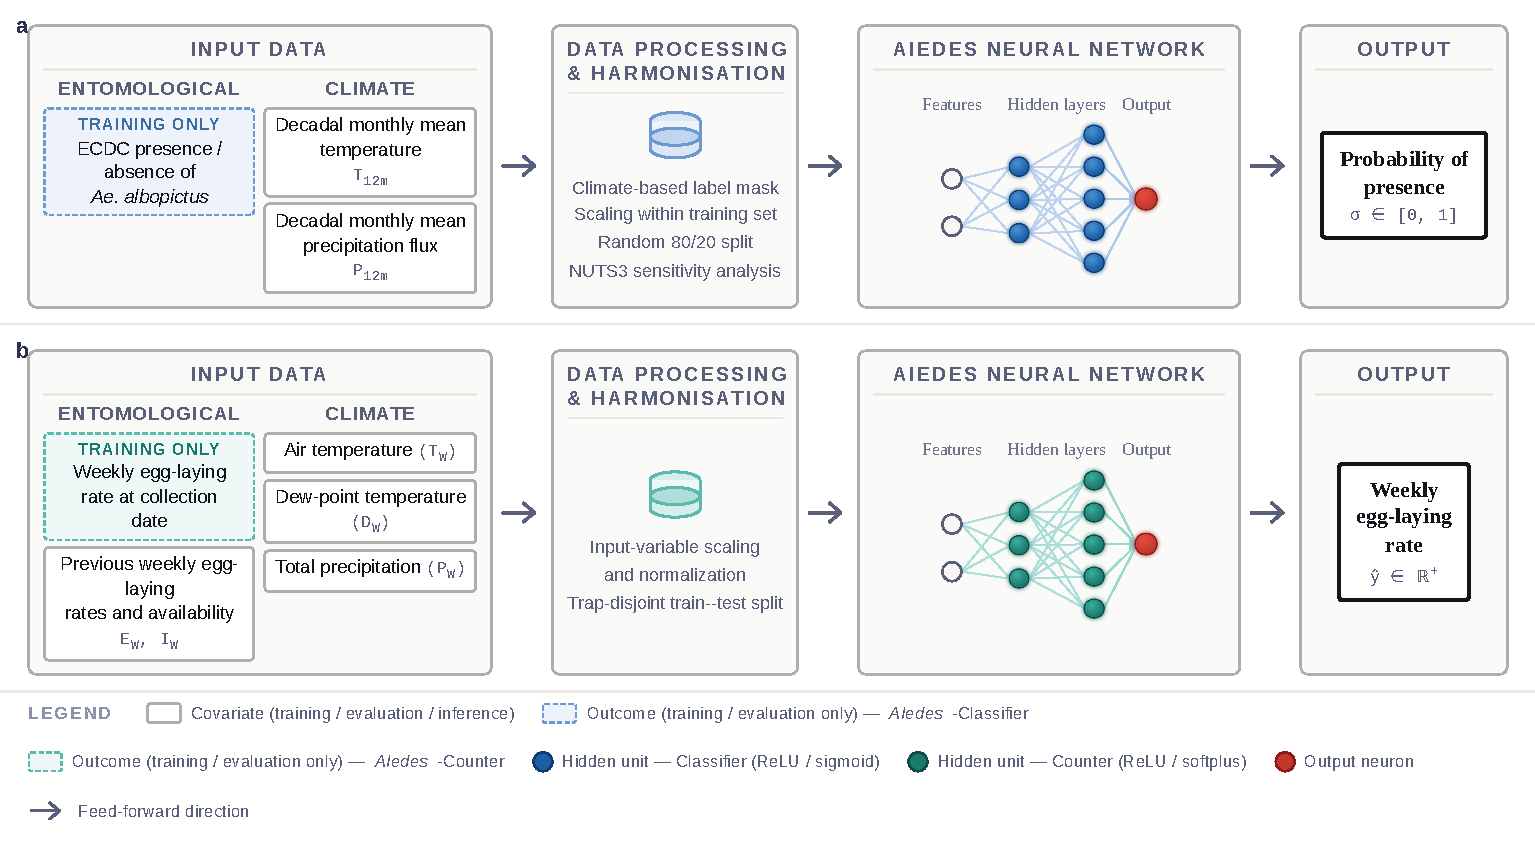
\includegraphics[width=\linewidth]{img/concept_model_panel.pdf}
    \caption{Schematic representation of the Feed-Forward Neural Network (FFNN) architecture for the two components of \textit{\textbf{AI}edes}. \textbf{(a)} \textit{\textbf{AI}edes}-Classifier: the network takes as input decadal monthly averages of 2-m air temperature ($AT_{12m}$) and total precipitation flux ($MP_{12m}$), alongside presence/absence labels used exclusively during training, and outputs a habitat suitability index $\sigma \in [0,1]$ via a sigmoid activation. \textbf{(b)} \textit{\textbf{AI}edes}-Counter: the network takes as input 90-day daily time series of air temperature ($AT_{90d}$), dew point ($DP_{90d}$), and total precipitation ($TP_{90d}$), optionally augmented by the two preceding weekly egg-laying rates ($ER_{2w}$) when available, and outputs a weekly egg-laying rate $\hat{y} \in \mathbb{R}^+$ via a softplus activation. Both architectures share the same general FFNN structure, illustrated here with two hidden layers of 3 and 5 nodes respectively; hidden layers use ReLU activations. Arrows indicate the feed-forward direction of information flow.}
    \label{fig:concept_model}
\end{figure}

\textit{\textbf{AI}edes} is a neural network-based model comprising two components: \textit{\textbf{AI}edes}-Classifier and \textit{\textbf{AI}edes}-Counter. The first calculates the probability of presence of \emph{Ae. albopictus}, while the second estimates their abundance. 
They are implemented in Python using the PyTorch framework \cite{paszke2019pytorch}; the code and the final neural network model are freely accessible in \cite{github2024aiedes}; the curated datasets are described and released in \cite{biazzo2026_datasets}. 
We partitioned the datasets into a training set, representing $80\%$ of the available data, and a test set consisting of the remaining $20\%$, used for performance evaluation.  \\

Figure \ref{fig:concept_model} shows a schematic representation of the general Feed-Forward Neural Network (FFNN) architecture used for both components to estimate the probability of the presence and abundance of \emph{Ae. albopictus} based on climate and biological variables in a given location. The figure illustrates a network with two hidden layers comprising 3 and 5 nodes, respectively; the arrows show the direction that the output of the previous step follows to feed forward into the nodes of the following step or layer.



\subsubsection{\textit{\textbf{AI}edes}-Classifier}

\begin{comment}
\begin{figure}
    \centering
    \includegraphics[width=0.75\linewidth]{img/FFNN_simple.PNG}
    \caption{
    Schematic representation of the general feed-forward neural network (FFNN) architecture used for the \textit{\textbf{AI}edes}-Classifier to estimate the probability of presence of \emph{Ae. albopictus} based on climate variables at a given location. The figure illustrates a network with two hidden layers comprising 3 and 4 nodes, respectively ([3, 4]), and an output layer with a sigmoid activation function, ensuring that the output is constrained between 0 and 1. Notably, when no hidden layers are present, an FFNN with a sigmoid output layer is mathematically equivalent to logistic regression.}
    \label{fig:FFNN_simple}
\end{figure}
\end{comment}



The goal of the \textit{\textbf{AI}edes}-Classifier module is to predict the probability of presence  of \emph{Ae. albopictus} across Europe in a given calendar year. The input variables consist of monthly climatic measurements, aggregated from the original hourly data: temperature and precipitation. The model outputs a value between 0 and 1, which represents the probability of \emph{Ae. albopictus} being present at a given location during a calendar year. By convention, a predicted probability greater than $0.5$ is considered indicative of the presence of \emph{Ae. albopictus}, while a probability of $0.5$ or lower is interpreted as absence.

The hidden layers use the ReLU (Rectified Linear Unit) activation function, while a sigmoid activation function is applied to the final output to constrain predictions within the [0,1] range. Notably, when no hidden layers are present, an FFNN with a sigmoid output layer is mathematically equivalent to logistic regression. As previously described, both input climate variables and presence/absence data are split into training and test datasets (in proportion 80:20); with only the latter used to compute the performance metrics.
The model is trained using the binary cross-entropy loss function \cite{bishop2006pattern} and optimized with the Adam optimizer \cite{kingma2014adam}, with a learning rate of 0.001. 

\begin{figure}
    \centering
    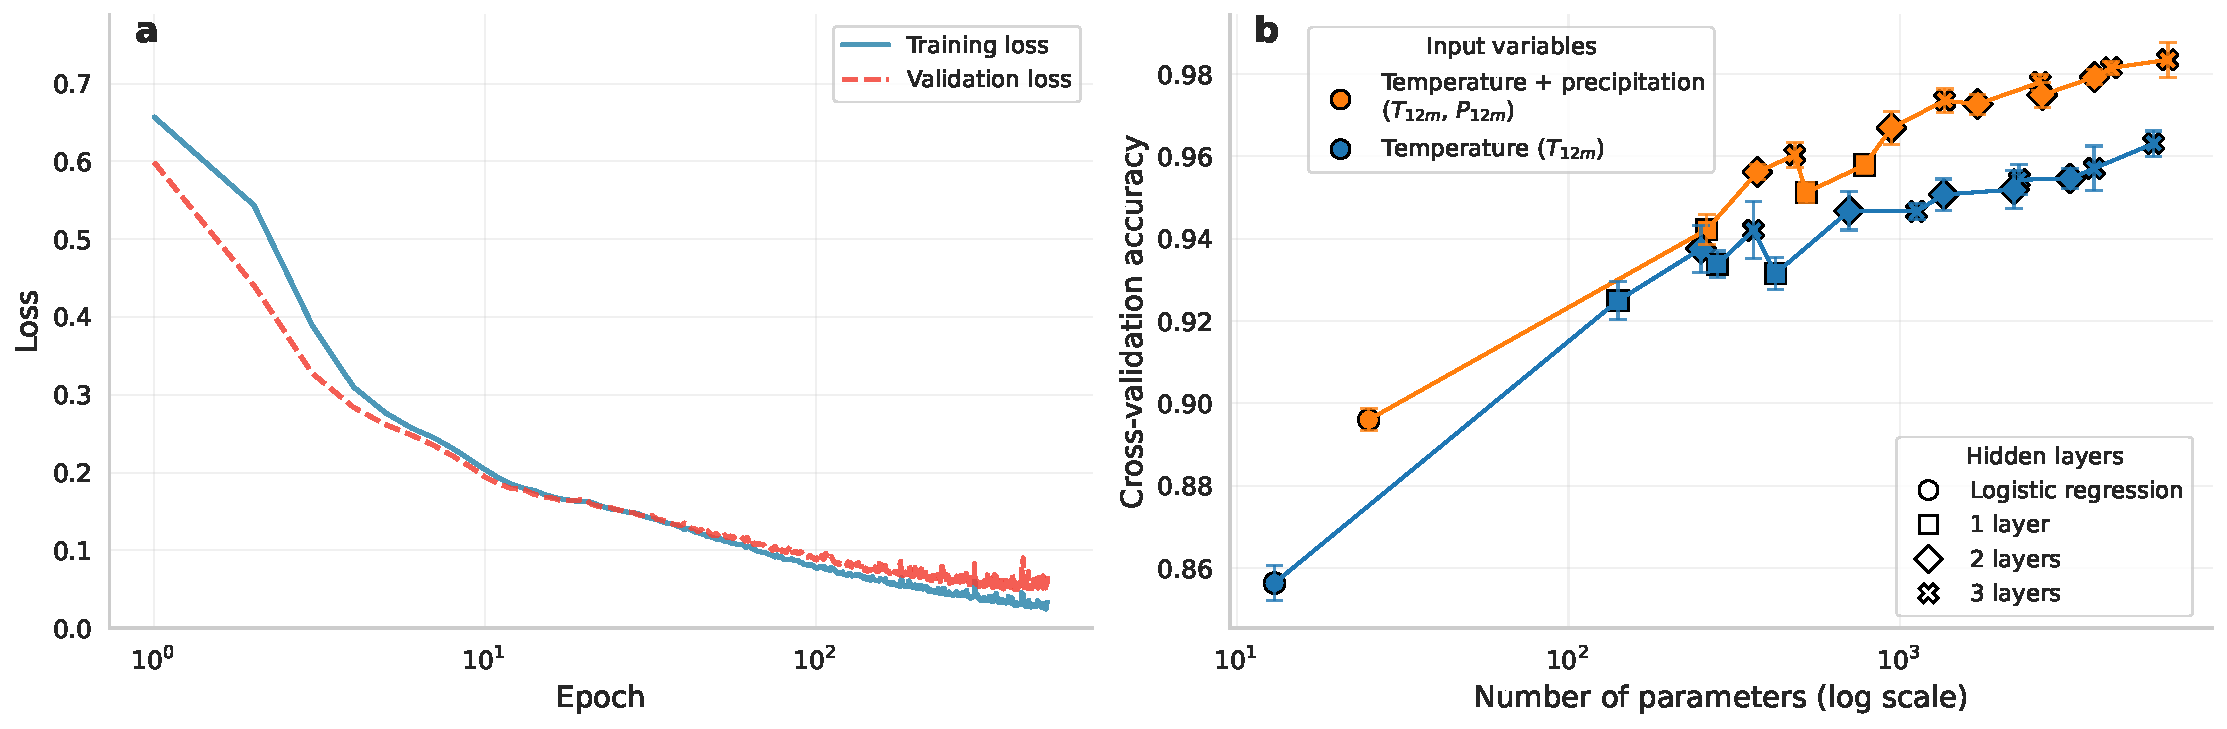
\includegraphics[width=1\linewidth]{img/combined_loss_acc.pdf}
    \caption{
\textbf{Training Dynamics and Model Performance of \textit{\textbf{AI}edes}-Classifier} \textbf{(a)} Example of training and testing loss curves over the training epochs for a neural network model (\textit{inputs}: temperature and total precipitation; \textit{architecture}: $[50,\,50]$, i.e., two hidden layers with $50$ nodes, or units, each). The dataset consists of $45{,}724$ data points, split into $80\%$ for training and $20\%$ for testing. The loss decreases and stabilizes after the initial epochs, with the testing loss remaining slightly higher than the training loss, indicating absence of overfitting.
    \textbf{(b)} 
    Accuracy computed on the test dataset for two types of input variables:  temperature only and temperature plus precipitation as a function of the total number of model parameters (on log scale). Points on the graph feature  different neural network architectures, i.e. different number of hidden layers (from $0$ - no hidden layer, equivalent to logistic regression, up to $3$ hidden layers). The number of parameters depends on the number of hidden layers and the number of units per layer. Increasing the number of units and layers, and including precipitation as an input further enhances accuracy.}
    \label{fig:loss_training}
\end{figure}

Figure \ref{fig:loss_training}a illustrates the typical behavior of the training and test loss functions over epochs. To optimize model performance, we conducted a series of tests varying both the number of hidden layers and the number of units per layer (Figure \ref{fig:loss_training}b). Architectures ranged from no hidden layers (equivalent to logistic regression) to configurations with up to three hidden layers containing 50 units each.
We evaluated model performance using the accuracy metric, considering two combinations of input variables: (i) monthly averaged temperature only, and (ii) monthly averaged temperature together with monthly total precipitation.

%Initially, we employed only the four \textbf{climate} [[bioclimatic]] variables, as described earlier, and subsequently incorporated monthly average temperature as an additional input to our neural network. 
The results, shown in Figure~\ref{fig:loss_training}b, indicate that increasing the number of layers and hidden units (and thus the total number of parameters) continues to yield performance gains, even at the highest tested values. However, the improvements become increasingly marginal and, as illustrated by the log-scaled x-axis, these small gains require exponentially larger increases in the number of parameters.

%and [[we]] clearly improves with respect \textbf{to} the performance of the logistic regression proposed in the paper [ref]. 
The inclusion of both monthly average temperature and total precipitation significantly improved the predictive accuracy, leading to an accuracy value close to $99\%$  for the model featuring the highest number of hidden layers and parameters. This is therefore the final model configuration chosen for testing (see Results section).

\subsubsection{\textit{\textbf{AI}edes}-Counter}
The \textit{\textbf{AI}edes}-Counter module is designed to predict the weekly egg-laying rate of \emph{Ae. albopictus} collected using ovitraps, as defined in the AIMSurv project, using climate variables from previous periods at each specific location.

As previously described, $80\%$ of the AIMSurv dataset is used for training (4.345 data points). 
The input variables consist of key climatic and biological factors sourced from the Copernicus programme (see Data section).

The model estimates the weekly egg-laying rate using a Weighted Mean Squared Logarithmic Error (WMSLE) loss function to address the data imbalance arising from the fact that approximately $80\%$ of the dataset consists of zero values (no eggs detected). We further tested alternative loss functions, such as a zero-inflated negative binomial loss designed to address data skewness; additional details are provided in the Supplementary Information.

We used feed-forward neural networks varying the number of hidden layers and the number of units per layer. All hidden layers used ReLU activation, while a final softplus function was applied to ensure strictly positive output rates. We tested several combinations of input variables.
We performed extensive hyperparameter optimization by varying the dropout rates, the number of hidden layers, and the number of units per layer. 
In contrast to the classifier, the training dataset used here contains almost ten times fewer data points, while the number of input variables is substantially higher. To preserve the expressivity of the model, the neural network therefore requires more parameters, which in turn makes the risk of overfitting considerably higher than in the AIedes classifier case.

For this reason, dropout regularization \cite{srivastava2014dropout} played an especially important role in mitigating overfitting. For each configuration, we conducted 20 independent runs using different random splits of the training and test sets. Model performance was compared based on the average $R^2$ on the test sets. To reduce the influence of poorly trained or overfitted runs, we retained only the top $25\%$ of $R^2$ values for each configuration—excluding both underperforming model trainings and extreme overfitting cases. These filtered results are reported in Fig.~\ref{fig:counter_input_var}.

\begin{figure}[h]
\centering
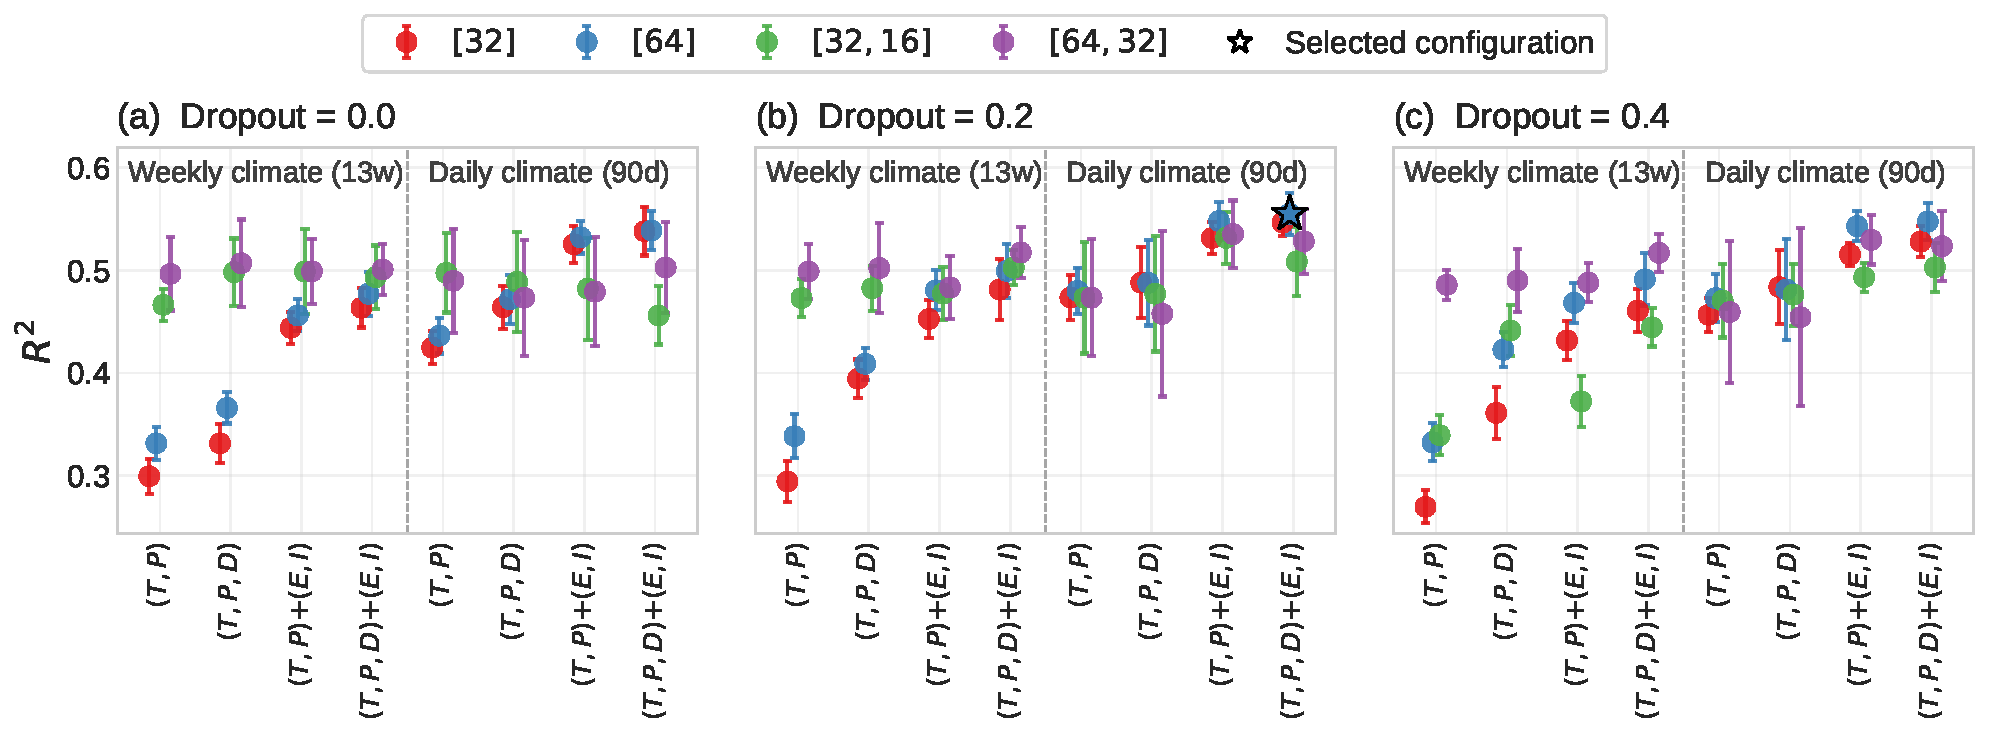
\includegraphics[width=1\linewidth]{img/nn_results_by_dropout.pdf}
\caption{
Predictive performance ($R^2$ score) of neural network models for weekly egg-laying rates of \emph{Ae. albopictus} as a function of input variables, dropout rates, and network architectures. Tested predictors include lagged egg-laying rates ($ER_{2w}$), daily averages of air temperature ($AT_{90d}$), total precipitation ($TP_{90d}$), and dew point temperature ($DP_{90d}$) over the 90 days preceding egg collection, as well as their weekly-averaged counterparts ($AT_{13w}$, $TP_{13w}$, $DP_{13w}$). Models using daily inputs ($AT_{90d}$, $TP_{90d}$, $DP_{90d}$) consistently outperform those based on weekly averages, although appropriate regularization through non-zero dropout values is necessary to mitigate overfitting. The best predictive performance is obtained with all variables, further improved by lagged egg-laying rates; this configuration, highlighted with a $\star$ in the figure, is taken as our \textit{\textbf{AI}edes-Counter}.
}
\label{fig:counter_input_var}
\end{figure}


Results indicate that model performance generally improves with the inclusion of additional input variables, though gains diminish once three variables are reached. When the previous two weekly egg counts were included alongside the three climate variables, performance improved further, highlighting the predictive value of recent temporal dynamics. The best-performing configurations demonstrate that applying an appropriate level of dropout was essential to reduce overfitting. Using weekly averaged input variables led to worse performance compared to daily inputs, suggesting that the potential benefit of simpler neural networks (and thus reduced overfitting) was offset by the loss of temporal information crucial for predictive accuracy.

Tab.~\ref{tab:top5models} reports the five best model configurations ranked by mean $R^2$. Although the loss function (WMSLE) ranking does not exactly coincide with the $R^2$ ranking, all discrepancies lie within the corresponding standard errors, indicating statistical compatibility. The table also shows the mean classification accuracy for presence/absence. Despite minor reordering across metrics, all top configurations display consistent, robust performance, supporting the chosen input variables and architectures.

\begin{table}
\centering
\footnotesize
\caption{Top five Neural Network configurations, ranked by mean $R^2$
 score. The mean is calculated from the five best-performing runs out of ten total runs for each configuration.
Each row reports the input variables used, dropout rate, number of hidden layers (Lay), number of units per layer (HU), along with the mean and standard error (SE) of the $R^2$, root mean square error (RMSE), and classification accuracy (Acc) for presence/absence (i.e., zero vs.~non-zero egg counts). All models were trained to predict weekly egg counts of \emph{Ae. albopictus} using climatic and historical egg-laying data.}
\label{tab:top5models}
\begin{tabular}{lcrrrrrr}
\toprule
Variables & DO & Lay & HU & $R^2$ & Loss & Acc & RMSE \\
\midrule
$AT_{90d}$\,\text{+}\,$TP_{90d}$\,\text{+}\,$DP_{90d}$\,\text{+}\,$ER_{2w}$ & 0.2 & 2 & 64 & $0.627 \pm 0.006$ & $0.59 \pm 0.02$ & $0.920 \pm 0.002$ & $22.6 \pm 1.3$ \\
$AT_{90d}$\,\text{+}\,$TP_{90d}$\,\text{+}\,$DP_{90d}$\,\text{+}\,$ER_{2w}$ & 0.0 & 2 & 64 & $0.626 \pm 0.014$ & $0.63 \pm 0.04$ & $0.919 \pm 0.001$ & $23.4 \pm 1.9$ \\
$AT_{90d}$\,\text{+}\,$TP_{90d}$\,\text{+}\,$DP_{90d}$\,\text{+}\,$ER_{2w}$ & 0.4 & 2 & 64 & $0.619 \pm 0.005$ & $0.59 \pm 0.04$ & $0.920 \pm 0.001$ & $22.9 \pm 1.3$ \\
$AT_{90d}$\,\text{+}\,$TP_{90d}$\,\text{+}\,$ER_{2w}$ & 0.2 & 2 & 64 & $0.617 \pm 0.008$ & $0.60 \pm 0.04$ & $0.921 \pm 0.002$ & $22.9 \pm 1.4$ \\
$AT_{90d}$\,\text{+}\,$TP_{90d}$\,\text{+}\,$ER_{2w}$ & 0.4 & 2 & 64 & $0.616 \pm 0.010$ & $0.57 \pm 0.03$ & $0.922 \pm 0.001$ & $22.9 \pm 1.2$ \\
\bottomrule
\end{tabular}
\end{table}

For the analyses that follow, we adopt the top-ranked configuration in Tab.~\ref{tab:top5models}, which uses as inputs the daily air temperature, total precipitation, and dew point over the preceding 90 days ($AT_{90d}$, $TP_{90d}$, $DP_{90d}$), together with the two-week aggregated egg-laying rate ($ER_{2w}$) when available. The selected network has two hidden layers with 64 units each (HU = 64, Lay = 2) and dropout $=0.2$. Among the 5 runs trained shown for this configuration, we choose the instance whose $R^2$ is closest to the configuration’s mean to provide a representative, unbiased model.


\section{Results}

\subsection{Predicting Local Mosquito Presence and Absence}

Here we present the results of the \textit{\textbf{AI}edes}-Classifier model, trained on presence and absence data. For this analysis, the selected input variables are monthly average temperature and total precipitation, as described in Methods. Figure~\ref{fig:nn_accuracy_map} compares predictions from the simplest neural network tested - a model with no hidden layers, statistically equivalent to logistic regression (Fig 4a) - and those from the best-performing architecture, consisting of three hidden layers with 50 units each (Fig 4b). These models predict the geographical distribution of \textit{Ae. albopictus} using observational data (see Data section). The input variables are monthly decadal averages of temperature and total precipitation values over the decade 2011–2020, derived from the Copernicus dataset.


The output of these models is the probability of presence for \textit{Ae. albopictus}, where probabilities above 0.5 are interpreted to indicate predicted presence and probabilities below 0.5, to indicate absence. Our best performing model achieves high accuracy (0.988) on the test dataset. It shows particularly high sensitivity (0.983), specificity (0.991) and CSI (0.974), indicating excellent overlap between predicted and observed distributions. In contrast, logistic regression, similar to models used in earlier studies (e.g. \cite{zardini2024}), only captures simpler spatial patterns, leading to higher levels of prediction error. For example, sizable areas of Spain, France, Central Europe and the Balkans are classified falsely as negatives by this model. A more detailed comparison of our best performing model to the logistic regression model is provided in the Supporting Information. The deeper neural network shows clear improvements over the simpler model. The results confirm that the improvement in accuracy observed here with Copernicus-derived inputs is consistent with the gains obtained under that earlier input setting.
To assess the robustness of these results to potential spatial autocorrelation in the Copernicus-derived inputs, we additionally performed a sensitivity analysis in which training and test data were separated at the NUTS3 regional level rather than by random point-wise splitting. As expected, this more stringent spatial separation leads to slightly reduced but still high performance metrics. These additional analyses, which confirm the stability of the results, are reported in the Supporting Information.


\begin{figure}[h]
    \centering
    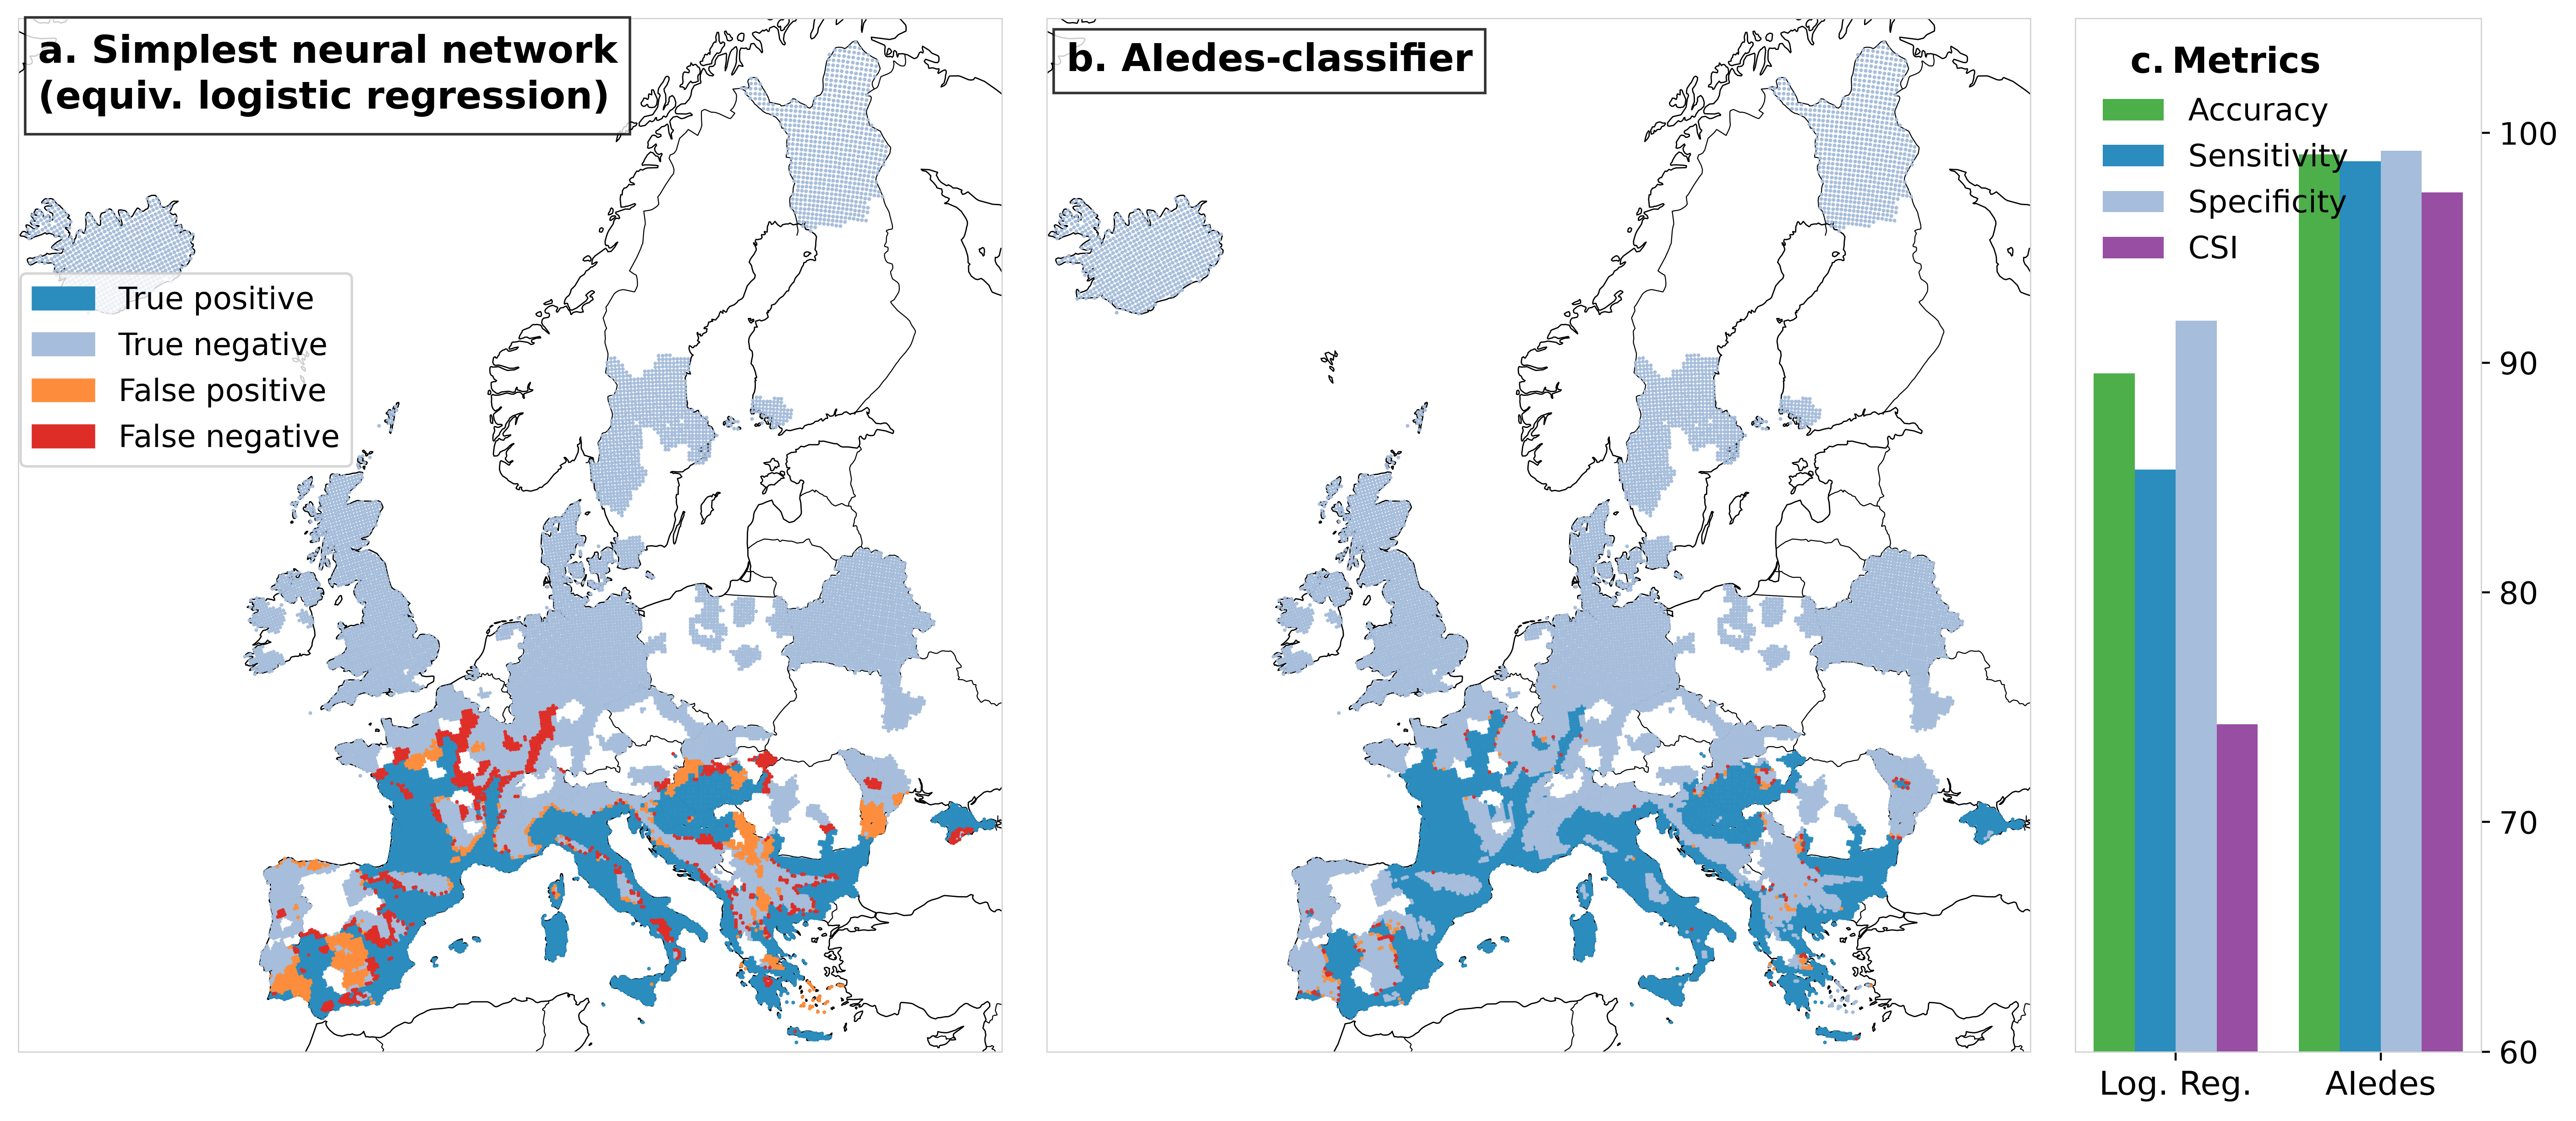
\includegraphics[width=0.95\textwidth]{img/comparison_lr_nn.png}
    \caption{Predicted probability of presence of \textit{Ae. albopictus} using the \textit{\textbf{AI}edes}-Classifier in comparison to the observed presence of the species.
a. Predictions from the simplest neural network architecture tested, featuring no hidden layers, equivalent to logistic regression. b. Predictions from the best-performing model, which features three hidden layers with 50 units each. c. Performance metrics of both models compared to observed data: accuracy, sensitivity, specificity and critical success index (CSI). }
    \label{fig:nn_accuracy_map}
\end{figure}



\subsection{Abundance Predictions}

\begin{figure}[h]
\centering
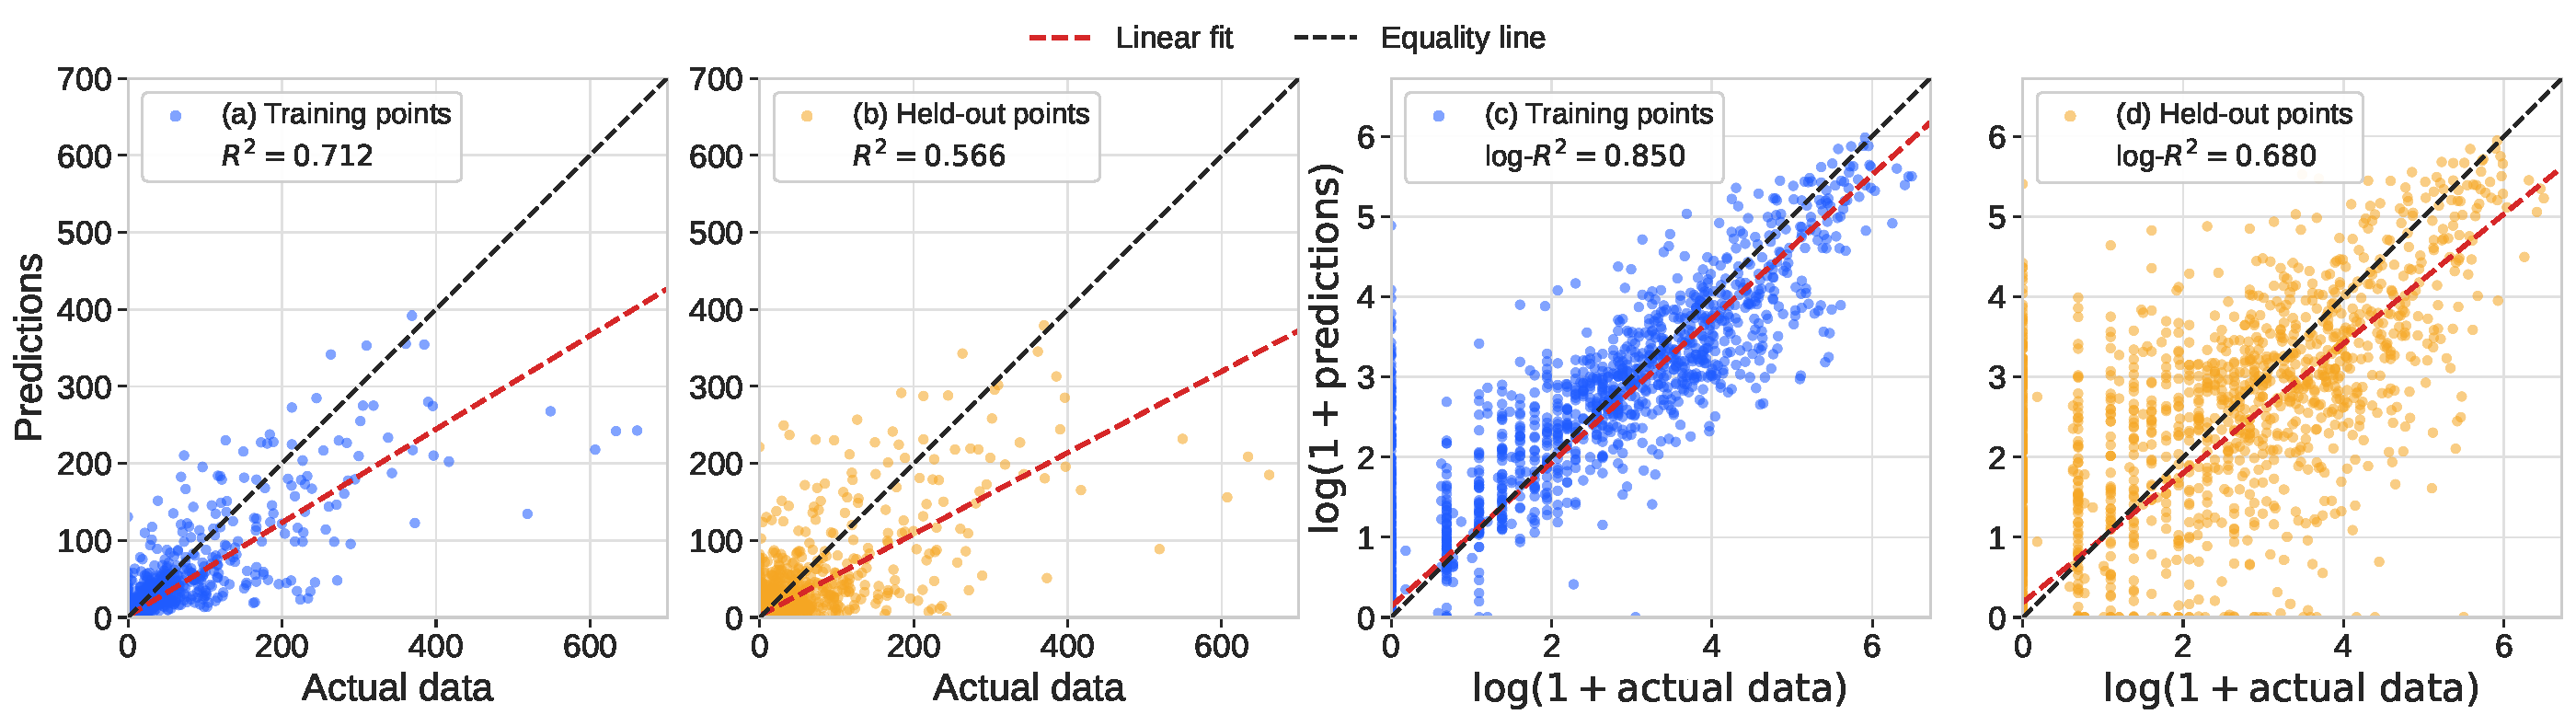
\includegraphics[width=1\linewidth]{img/R2_scatter_plot.pdf}
\caption{Scatter plots of actual versus predicted weekly egg counts for the training dataset (a) and the testing dataset (b). Points lie slightly below the bisector, suggesting a mild underprediction; however, results from the Bland–Altman test (see Supplementary Information) confirm that this is not a systematic bias.} 
\label{fig:r2}
\end{figure}

The scatter plot in Figure \ref{fig:r2} compares the actual and predicted weekly egg counts derived from the best combination of input variables and neural network architecture: we used $AT_{90d}$, $TP_{90d}$, $DP_{90d}$ (see Table \ref{tab:inputs_var}), together with the previous one and two-week aggregated egg-laying rates $ER_{2w}$, within a 2 hidden layers NN architecture with a total of 64 units per layer. Panel (a) shows the results for the training dataset, and panel (b) shows the results for the testing dataset. The comparison demonstrates an overall good predictive accuracy and only minimal overfitting. The high $R^2$ values ($R^2_{train}=0.68$, $R^2_{test}=0.63$) indicate a good predictive performance of our model. The similarity of the $R^2$ values across the training and test datasets indicates that the neural network has been successful in capturing important trends and associations between input and output data, and that the model has learned the key biological and environmental relationships. It further suggests that the test dataset is representative of the conditions under which the model was trained. Although the fitted values tend to lie slightly below the bisector, suggesting a potential underprediction bias, results from the Bland–Altman test (see Supplementary Information) confirm that this deviation does not reflect a systematic underestimation.


\begin{figure}[h]
\centering
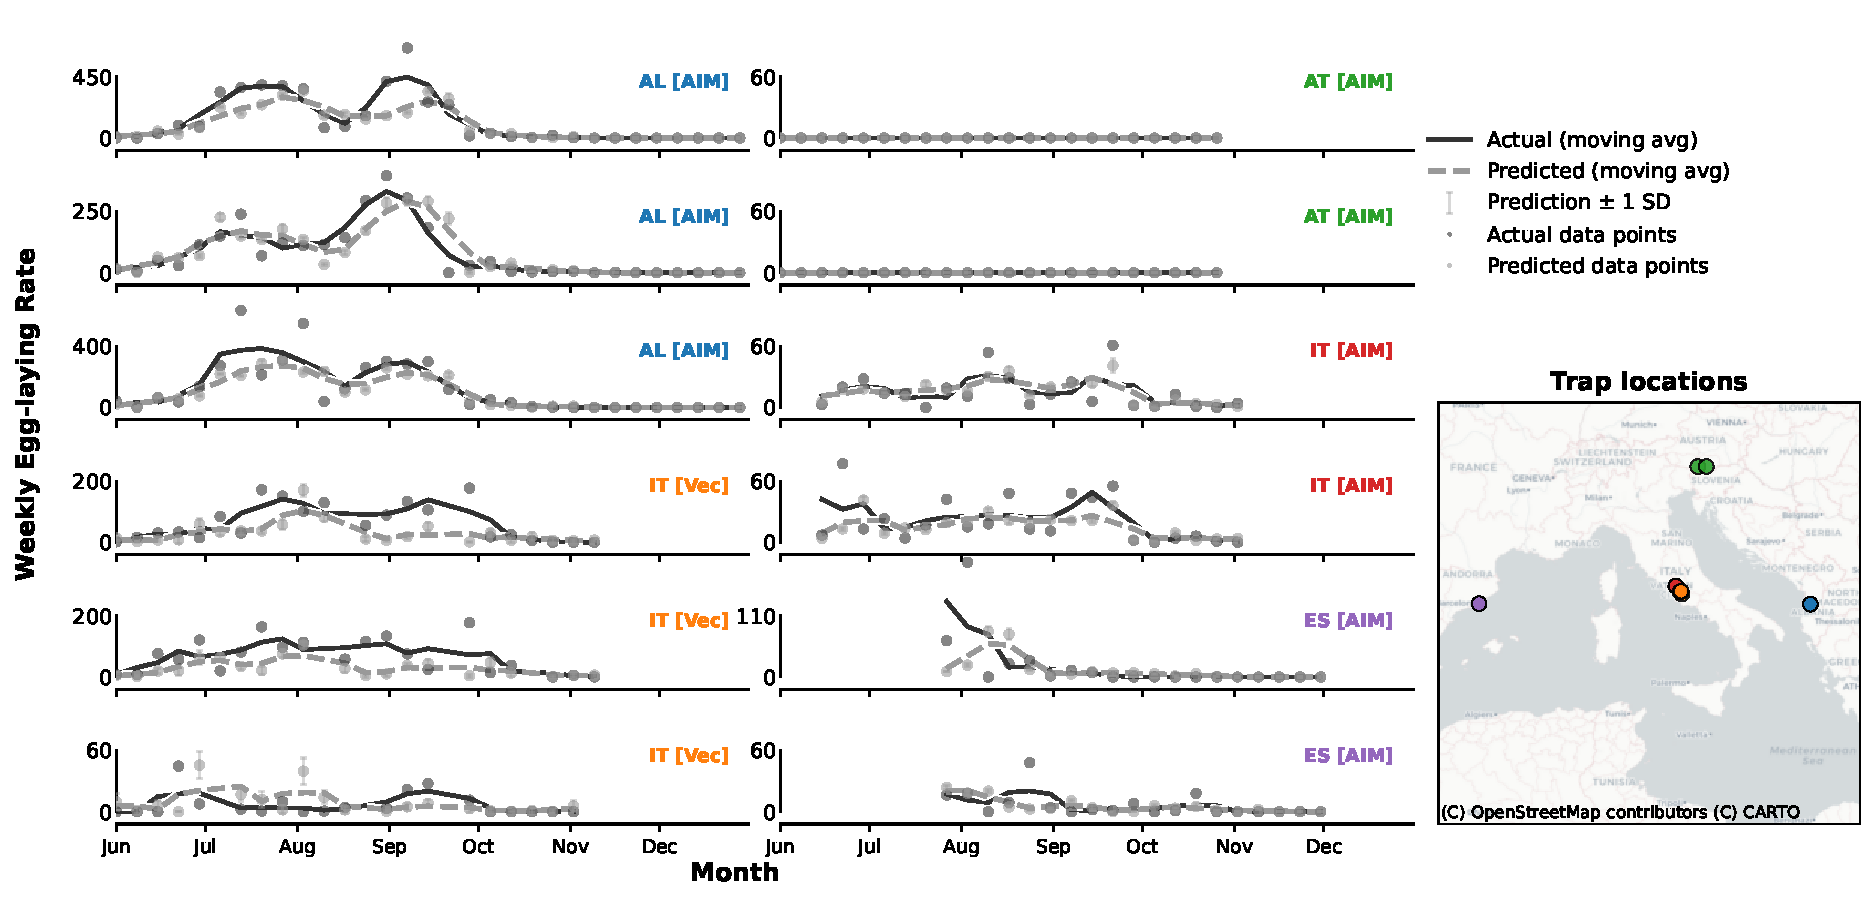
\includegraphics[width=1\linewidth]{img/most_populated_traps_time_series.pdf}
\caption{
Observed and predicted weekly egg counts from selected traps across 4 countries from the AIMSurv and VectorNet datasets. Data points show observed and predicted weekly mosquito egg-laying rates counts. Superimposed curves represent a centered rolling average (window size = 3) highlighting temporal trends. Circles represent data points from the training set, squares represent those from the test set. Note that the y axes differ across graphs.}
\label{fig:time_series}
\end{figure}

\begin{figure}
    \centering
    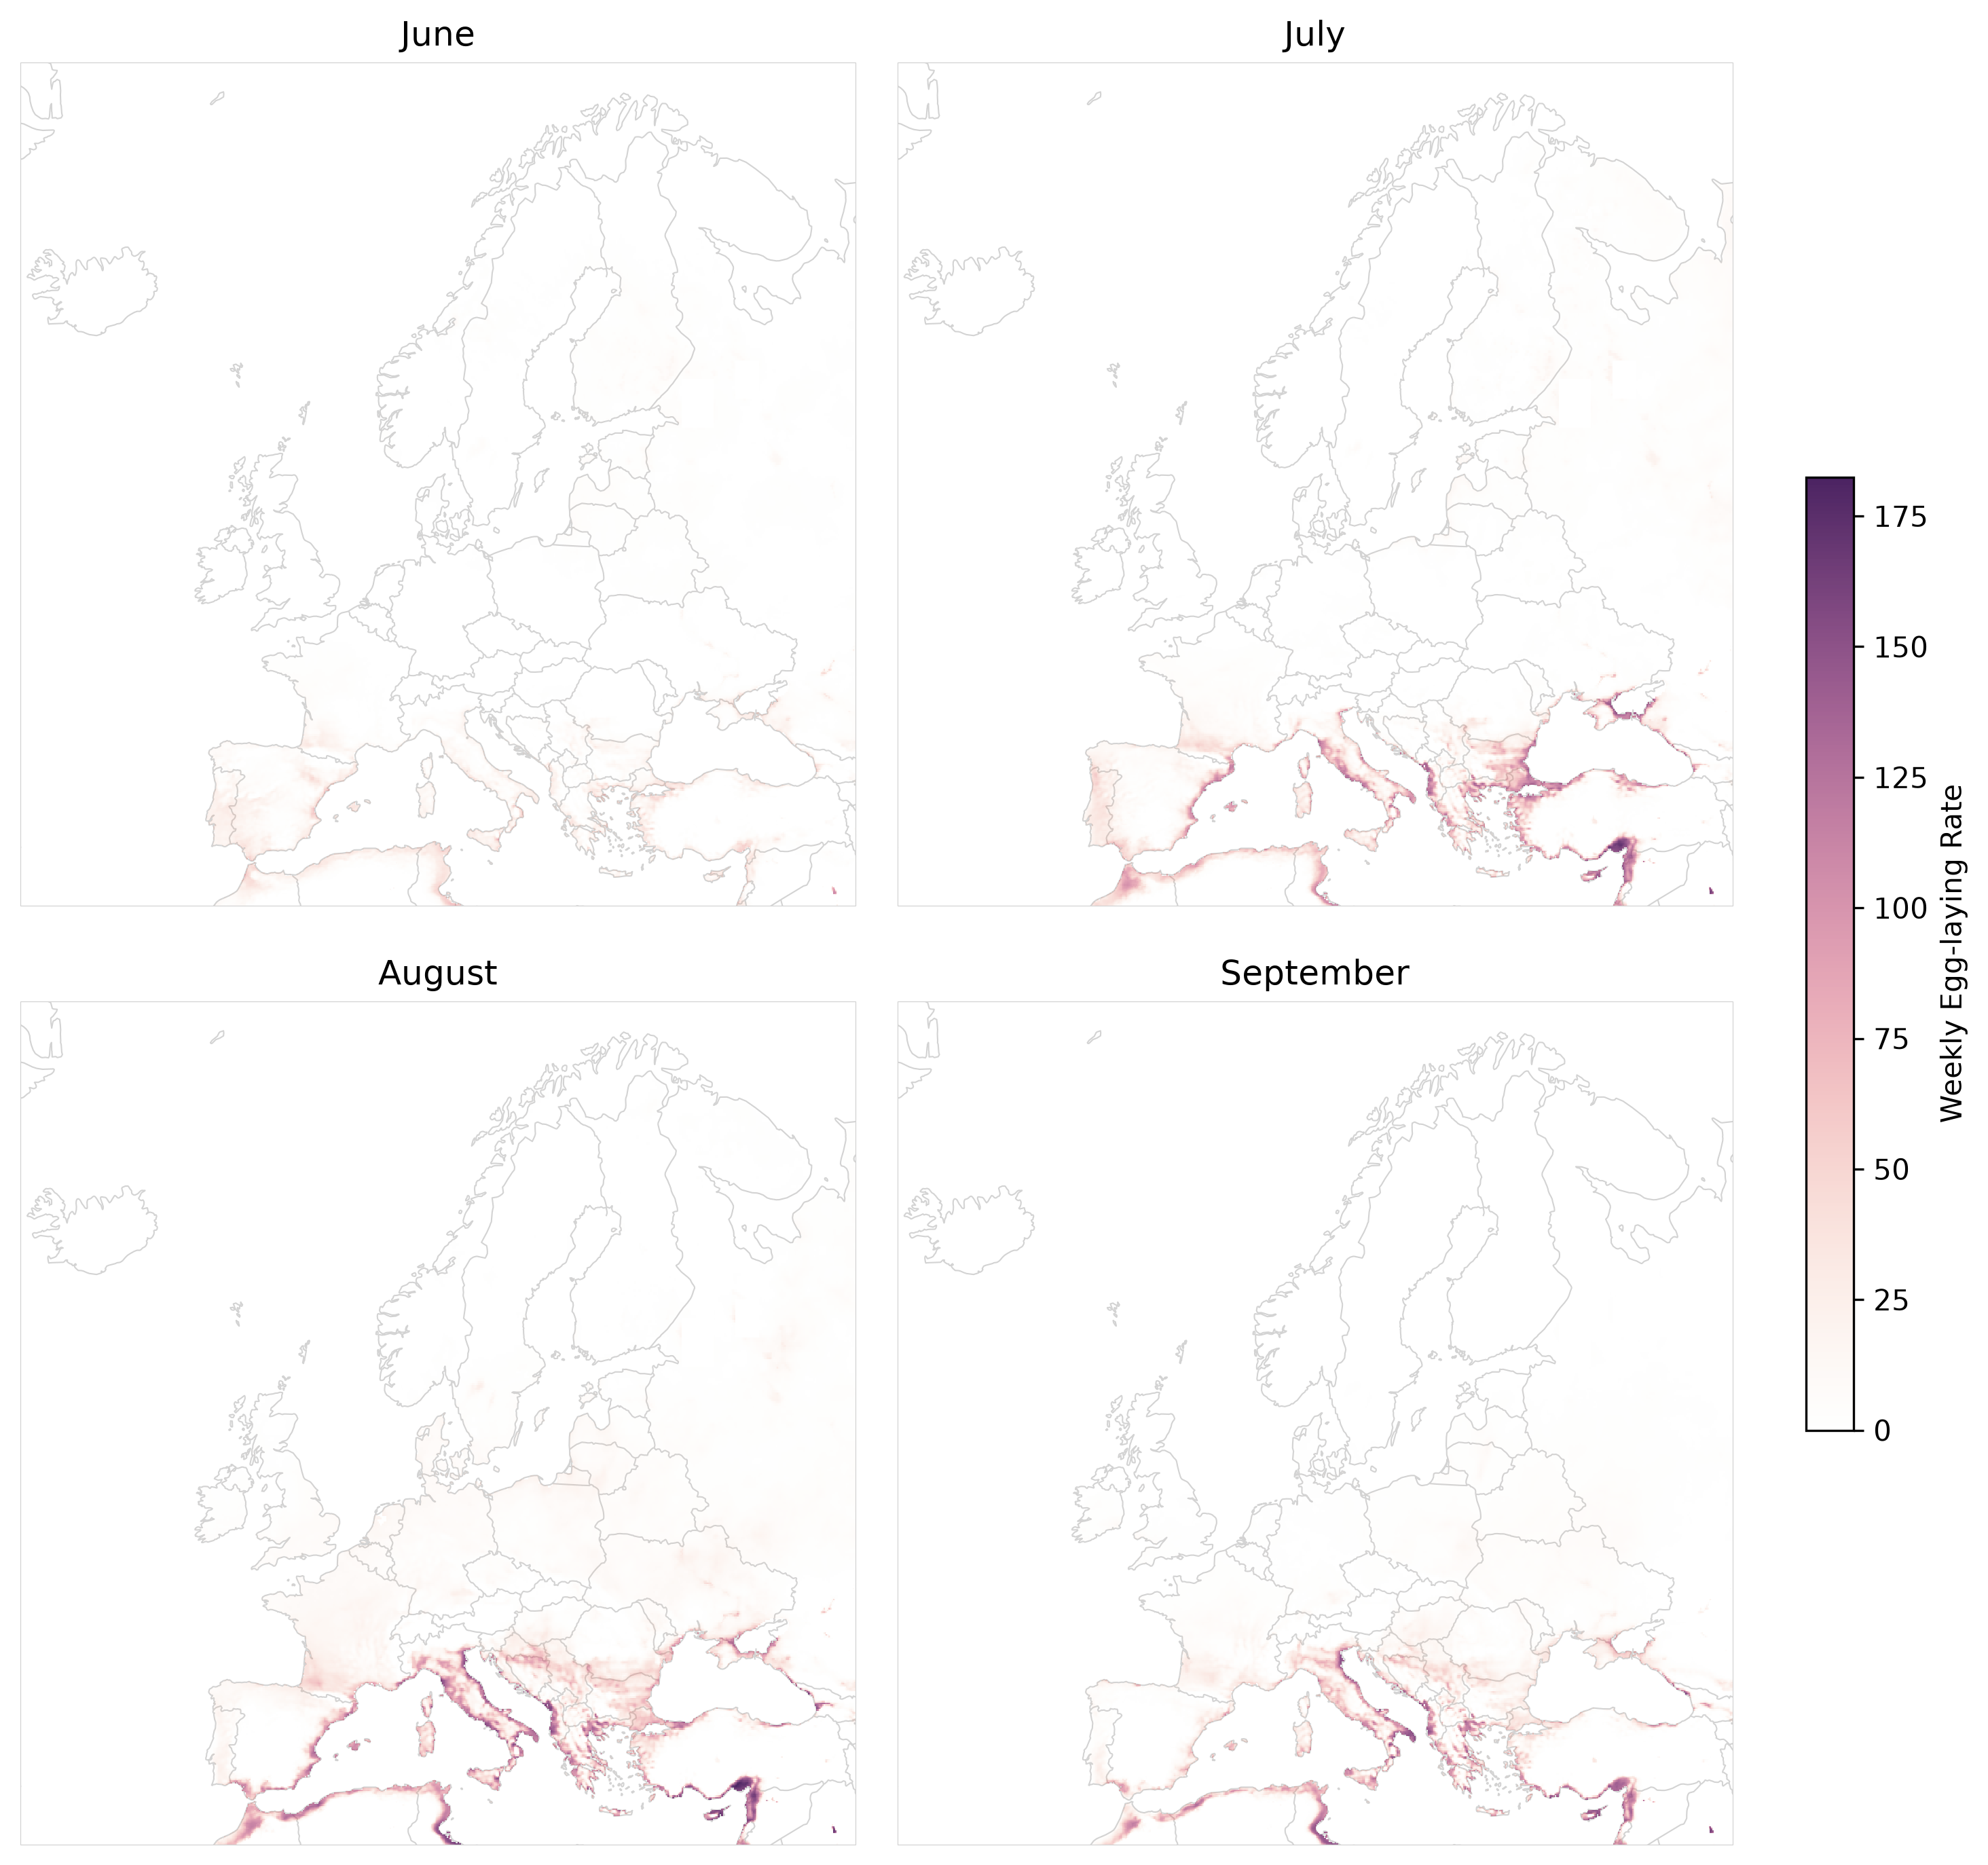
\includegraphics[width=1\linewidth]{img/weekly_rates_map.png}
\caption{
Predicted average egg-laying rates of \textit{Ae. albopictus} across Europe during the peak mosquito season for the months June–September of 2020. The maps display the monthly averages of weekly predictions, capturing the core period of the mosquito reproductive season, highlighting spatial and seasonal variation in predicted mosquito abundance. 
}
\label{fig:enter-label}
\end{figure}

Figure~\ref{fig:time_series} displays time series of weekly egg-laying rates from selected traps, comparing the actual observed values to the corresponding predictions of the \textit{\textbf{AI}edes}-Counter model. The figure presents nine time series from the AIMSurv dataset and three from the ECDC/EFSA VectorNet dataset. For each dataset, we selected the traps with the longest available time series, with a maximum of three traps per country. For VectorNet, the only data meeting our selection criteria were from Italy in 2021, as detailed in the Materials and methods section. Within each subplot, the individual points represent the weekly egg-laying rates, with the actual observed and predicted values shown separately. To help interpretation and to highlight overall trends, a moving average (window size = 3 weeks) is superimposed on both the observed and predicted series. The close correspondence between the predicted and observed moving averages, particularly in the AIMSurv series (benefiting from consistent sampling protocols), demonstrates the strong model performance across multiple time series and data sources.


Finally, Figure~\ref{fig:enter-label} presents the predicted average weekly egg-laying rates during the four central months of the 2020 \textit{Ae. albopictus} season in Europe. The modeling procedure begins by estimating the average weekly rate for each grid cell using only the climate variables for the first two weeks of the season. For all subsequent weeks, the model also incorporates an autoregressive component: predictions are generated by combining the climate variables of the given week with the egg-laying rates predicted for the previous weeks. This iterative process continues until the end of the calendar year. The maps report the spatial distribution of monthly averages of the predicted weekly rates for June through September, which correspond to the peak of the mosquito reproductive season. The maps display a clear progression from June to August, with mosquito abundance building substantially through the summer. As expected, August appears to represent the peak month in abundance across most regions, suggesting optimal breeding conditions. We can also observe an evident south-to-north gradient, with Mediterranean and southeastern European regions showing sustained high activity throughout September while northern areas of the continent remain largely unaffected throughout the entire period.\\




\section{Discussion}

The field of modeling vector mosquitoes' spatial distribution and abundance has long faced considerable challenges and limitations in developing comparable and reproducible approaches. Models are often applied to data on small spatial extents \cite{guzzetta2016, Kioutsioukis2019, angelou2021, dare2022, dare2025, kinney2024rapid}, rely on data sets and quantities that are not easily reproducible \cite{li2019}, or feature only qualitative analyses without robust performance metrics \cite{davis2024, zardini2024}. These limitations have made systematic comparisons across models difficult, especially for predicting vector abundance, where data are typically more scarce, heterogeneous, and collected under different protocols, not necessarily for the purpose of predicting vector abundance. In addition, models often predict non-comparable quantities and use code that is either unavailable or not user-friendly.

Recent developments in data availability and methodology have created new opportunities to improve the quality and reliability of mosquito vector distribution estimation. Thanks to efforts such as the ECDC mosquito presence maps and the AIMSurv European collaboration, large-scale datasets are now available, enabling among other things the application of novel and powerful machine learning approaches. Building on these advances, here we present \textit{\textbf{AI}edes}, a new, fully data-driven, validated and replicable approach for estimating mosquito presence and abundance using neural networks.\\

By combining the well-curated datasets from ECDC/EFSA VectorNet \cite{ecdc2024a}, the AIMSurv project \cite{miranda2022aimsurv}, and Copernicus climate data, we establish a framework that describes mosquito distributions on a continental scale and also applies rigorous validation and performance assessment via formal accuracy and $R^2$ statistics. This framework enables transparent evaluation and facilitates future comparisons with other modeling approaches using shared or comparable datasets.\\
%s.\\

Our \textit{\textbf{AI}edes}-Classifier model achieved excellent performance on the presence-absence task with accuracy of 98.8 \%, outperforming recently published model\cite{zardini2024}, while the \textit{\textbf{AI}edes}-Counter delivered strong results for abundance estimation by effectively predicting weekly egg-laying rates. Figure 4 shows that the sensitivity of the classifier model is more than 98\% while specificity is above 99\%. 

\textit{\textbf{AI}edes} Classifier is able to identify correctly both the overwhelming majority of grid cells where \emph{Ae. albopictus} is present and at the same time is not prone to incorrectly assigning presence in locations where the insect is absent.\\

Our best model limits areas with misclassifications to parts of Hungary, Serbia and Central Spain. A comparison with our map of estimated distribution of abundance (Figure 7) indicates that these areas feature very low expected number of mosquitoes, suggesting that the practical implications of such misclassification by the presence model would in fact be minimal.
\\

Similarly, for the \textit{\textbf{AI}edes} Counter model, the coefficient of determination values ($R^2_{train}=0.68$, $R^2_{test}=0.63$, Figure 5) indicate strong predictive performance, where the model is able to account for, and predict 63\% of the variability in local mosquito abundance across all geographical locations in our testing data set. From a model validation point of view, the similarity of the  of $R^2$ values across the training and testing run indicates low levels of overfitting, and so an optimal architecture of the employed neural network among those tested. It further suggests that the test dataset is representative of the conditions under which the model was trained. From a biological point of view this comparison shows that the model has successfully captured the cardinal trends and associations between input and output variables. 
Thirty-seven percent of the variation in the output data remains unexplained by the model. This residual variance is consistent with the intrinsically stochastic nature of mosquito population dynamics and egg-laying processes, which are subject to strong short-term and local fluctuations. Given the spatial and temporal resolution of the available climatic inputs, a non-negligible level of irreducible noise is therefore expected. Further reductions in unexplained variability would primarily require longer time series, increased temporal aggregation, and replicated observations, rather than the inclusion of additional deterministic predictors alone.

To demonstrate the strong performance of our model also at the level of individual time series, we present the data and estimates for a selection of the time series with longest follow-up periods (Figure 6). The close correspondence between the predicted and observed moving averages, demonstrates strong model performance across multiple time series and data sources. In the three VectorNet time series that fulfilled our selection criteria we observe that our model fails to capture the secondary peak in weekly egg counts occurring between September and October in each of the three recorded time series presented. The underlying reason is difficult to assess. All time series selected in VectorNet were collected as part of a separate elevation-focused study and do not follow the standardized and consistent AIMSurv sampling protocol. As a result, these time series are likely to reflect environments and methodology distinct from those underlying the AIMSurv dataset, and the relationships between input and output variables in this context may differ from the one captured during \textit{\textbf{AI}edes} training on AIMSurv data. Specifically, given the high altitude and location of the sampling sites, it is plausible that local micro-climatic conditions, especially in valleys or high-plateau environments, may not have been adequately represented in the training data set or insufficiently resolved in the climatic grid, which may have influenced mosquito abundance predictions.

Our predicted \textit{Ae. albopictus} egg laying rates for throughout Europe (Figure 7) exhibit a notable cline of increase of abundance towards southern Europe, a pattern consistent with climatic conditions in Europe's subtropical belts, much more suitable for breeding of the species. We also observe considerably higher vector abundance aggregations in the coastal areas of the Mediterranean, but also of the Black and Azov Seas further to the north. The four panels of Figure 7 also show that mosquito abundance exhibits a marked summer seasonal pattern with a peak during the months of July and August - the period of the year with higher day and night temperatures in combination with long periods of daylight. European countries positioned further north tend to peak in vector abundances later in the summer season, in August and even in September, as the most favourable weather conditions are likely reached later in these locations. 


In order for \textit{\textbf{AI}edes}-Classifier model to have public health utility, the next step would be to go beyond reproducing the current state of knowledge of \emph{Ae. albopictus} distribution status, and make predictions for those  areas where \emph{Ae. albopictus} is expected to be present in the absence of current surveillance data (e.g. in areas currently marked as 'no data' or 'unknown' in the map), so that surveillance can be targeted to those areas. A further step might even be to try to make distribution predictions for the future depending on climate change scenarios. However, life-history and ecological considerations will need to be taken into account when interpreting such maps of predicted \textit{Ae. albopictus} distribution in Europe: In the course of its migration to, and establishment in new areas in Europe the species is unlikely to have yet fully occupied its ecological niche across the continent. For instance, in the Netherlands, the species is not yet established despite suitable climatic conditions, due to active elimination efforts in the country. We excluded this region from our training dataset, however, similar situations may exist in locations where \textit{Ae. albopictus} is still in the process of expansion into new climatically suitable areas. Such locations are marked as negative not because of unsuitable conditions but because the invasion process is still incomplete. The species could therefore spread further under current climate conditions, potentially limiting the accuracy of predictions based on present-day distribution data.
A further methodological consideration concerns the construction of grid-level presence--absence labels. Our downscaling procedure inherits the limitations of NUTS3-level inputs combined with Copernicus climate predictors that are spatially autocorrelated. Neighbouring grid cells can therefore share both similar covariates and the same aggregated label. With an 80/20 random split, this structure can inflate performance estimates because correlated cells may enter both training and test sets. We adopted this setup to remain consistent with previous work and to enable a direct comparison of performance gains. Additional analyses using stricter spatial separation at the NUTS3 level yield qualitatively consistent results, suggesting that spatial autocorrelation does not drive the observed improvements (see Supporting Information).

Similarly, for the \textit{\textbf{AI}edes} Counter model, several considerations will need to be taken into account when interpreting predicted \textit{Ae. albopictus} population dynamics time series in Europe.
\textit{First}, the training data originate predominantly from regions with well-established surveillance programs, thus potentially introducing geographic bias toward areas with greater resources or heightened concern about mosquito-borne diseases. This may constrain model performance in under-sampled regions. For instance, the inability of our model to reproduce the secondary peak observed in a mountainous area of Italy may reflect an under-representation of such environments in the training dataset. 
\textit{Second}, the reliance on egg counts as a proxy for adult abundance may introduce additional uncertainty. Egg-laying, egg-hatching rates and successful transition through the development stages to an adult may vary with local conditions and mosquito behaviour not fully explained by climate variables alone and may correlate with adult population sizes in complex ways. These limitations underscore the need for more comprehensive and harmonized surveillance efforts, ideally covering multiple years, seasons, diverse ecological contexts, and multiple mosquito life stages.
In the best  \textit{\textbf{AI}edes}- Counter model, which included an auto-regressive component, observed egg counts two weeks prior in the same site informed the predictions. However, for the vast majority of practical situations where one would like to deploy a model to predict seasonally varying mosquito density, such leading observations are not available. For the generation of Figure 7, we deployed the model with a component auto-regressing on self-generated predictions, without using real egg count observations in the predicting process. A next step could be to evaluate time series of such predictions against  observed egg-count time series across Europe, and compare with competing models.
Models that can satisfactorily replicate observed mosquito population dynamics could then be combined with virus transmission models and disease importation data to inform public health about outbreak risks. 

An important further limitation concerning the \textit{\textbf{AI}edes} modelling approach (for both models) needs a mention. While neural networks deliver strong predictive performance, they provide limited interpretability, preventing straightforward identification of specific mechanistic phenomena, such as climate thresholds or factor interactions driving predictions. While our modelling framework does allow for assessment of the importance of input variables by examining changes in performance metrics on the testing dataset, this approach remains less informative than the more explicit parameter estimates and effect sizes provided by traditional statistical techniques.

With this work, we demonstrate in practice the effectiveness of neural networks---an approach that is at present underutilised for the modelling of the geographical distribution of vectors, both for presence-absence classification and for abundance prediction. Our methodology is based on recent advances in the AI community \cite{kraemer2025}, where benchmarking and standardized evaluation have accelerated progress across domains. To foster reproducibility and facilitate future comparisons, we release the code alongside ready-to-use datasets and detailed documentation, as a reference benchmark for the community \cite{github2024aiedes, biazzo2026_datasets}. Our approach integrates multiple high-quality data sources to predict both the probability of presence and the weekly abundance of \textit{Ae. albopictus} across Europe. With its diverse climatic conditions, different levels of mosquito establishment, and extensive surveillance programs, Europe provides a favourable setting for mosquito distribution modelling, yet, understandably, the methodology can be adapted to other regions, vector species, and to different spatial or temporal scales, provided adequate surveillance and environmental data are available.\\

Using two well-curated \textit{Ae. albopictus} datasets, we have shown the promise of data-driven approaches based on neural networks in ecological modeling and prediction. We anticipate that, in the coming years, with the accumulation of new datasets, the adoption of more advanced neural network techniques, and the integration of additional input variables---such as satellite imagery---results could improve even further and more rapidly. Future work should focus on expanding the model validation to additional regions and surveillance systems, improving confidence in model generalizability. Incorporating higher-resolution spatial data and additional environmental variables could refine predictive accuracy, while the integration of explainable AI methods or hybrid data-mechanistic approaches could enhance interpretability. Ultimately, combining robust AI-driven predictive tools with sustained investment in entomological surveillance will be essential to strengthen vector monitoring and support effective public health preparedness and control of mosquito-borne infections.

\section*{CRediT authorship contribution statement}

Indaco Biazzo: Conceptualization, Methodology, Software, Formal analysis,
Writing -- original draft, Writing -- review and editing.

Lia Orfei: Conceptualization, Methodology, Software, Formal analysis,
Writing -- original draft, Writing -- review and editing.

Ioannis Kioutsioukis: Conceptualization, Formal analysis,
Writing -- review and editing.

Lea Schuh: Conceptualization, Formal analysis,
Writing -- review and editing.

Céline Gossner: Formal analysis, Writing -- review and editing.

Olivier Briet: Formal analysis, Writing -- review and editing.

Peter V. Markov: Supervision, Conceptualization, Formal analysis,
Writing -- original draft, Writing -- review and editing.


\section*{Declaration of competing interest}

The authors declare that they have no known competing financial interests
or personal relationships that could have appeared to influence the work
reported in this paper.

\section*{Declaration of Generative AI and AI-assisted technologies in the writing process}

During the preparation of this work, the authors used GPT@JRC to support
language polishing and improve the clarity of the manuscript. After using
this tool, the authors reviewed and edited the content as needed and take
full responsibility for the content of the published article.

\section*{Funding}

This research did not receive any specific grant from funding agencies
in the public, commercial, or not-for-profit sectors.

\section*{Data and code availability}

The harmonised climate and \textit{Aedes albopictus} surveillance datasets
used in this study are publicly available through the European Commission,
Joint Research Centre Data Catalogue \cite{biazzo2026_datasets_doi}, DOI:
\href{https://doi.org/10.2905/e4e68952-a02f-460d-8f85-eb630742741d}
{10.2905/e4e68952-a02f-460d-8f85-eb630742741d}.
A detailed description of the dataset construction, harmonisation and
validation is provided in the companion data-descriptor manuscript submitted
to \textit{Scientific Data} \cite{biazzo2026_datasets}.
The source code, model implementation and documentation are available at
\cite{github2024aiedes}. The raw surveillance and climate data sources
used to construct the datasets are cited in the Materials and methods section.



\section*{Acknowledgements}
We would like to thank the colleagues of the Digital Health Unit (JRC.F7) at the Joint Research Centre of the European Commission for their guidance and support. 

The views expressed are those of the authors and may not in any circumstances be regarded as stating an official position of the European Commission. 

\bibliographystyle{elsarticle-num}
\bibliography{references}

\end{document}
